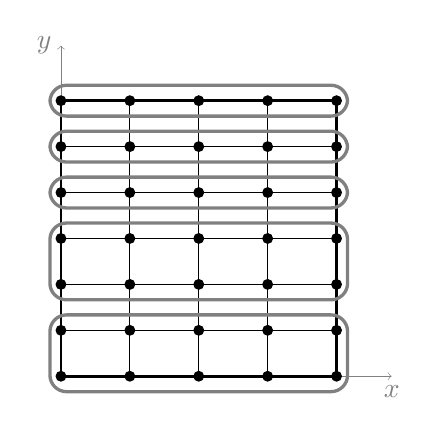
\begin{tikzpicture}[scale=3.5]
  \draw[->,gray,very thin] (0.0,0.0) -- (1.2,0.0) node[below] {$x$};
  \draw[->,gray,very thin] (0.0,0.0) -- (0.0,1.2) node[left] {$y$};
  \draw[line width=1.0pt] (0.0,0.0) -- (0.0,1.0) -- (1.0,1.0) -- (1.0,0.0) -- cycle;
  \pgfmathsetmacro\fourth{1.0/4.0}
  \pgfmathsetmacro\sixth{1.0/6.0}
  \draw[xstep=\fourth,ystep=\sixth,black,thin] (0.0,0.0) grid (1.0,1.0);
  \foreach \x in {0,...,4} {
    \foreach \y in {0,...,6} {
        \filldraw (\x * \fourth,\y * \sixth) circle (0.5pt);
    }
  }
  \pgfmathsetmacro\dd{0.04}
  \pgfmathsetmacro\od{1.04}
  \foreach \y in {0,2} {
    \pgfmathsetmacro\yup{\y * \sixth - 1.4 * \dd}  % less than 1.7 generates flaw?
    \pgfmathsetmacro\ydn{(\y + 1) * \sixth + 1.4 * \dd}
    \draw[very thick,rounded corners=6pt,gray] 
      (-\dd,\ydn) -- (\od,\ydn) -- (\od,\yup) -- (-\dd,\yup) -- cycle;
  }
  \foreach \y in {4,5,6} {
    \pgfmathsetmacro\yup{\y * \sixth - 1.4 * \dd}  % less than 1.7 generates flaw?
    \pgfmathsetmacro\ydn{\y * \sixth + 1.4 * \dd}
    \draw[very thick,rounded corners=6pt,gray] 
      (-\dd,\ydn) -- (\od,\ydn) -- (\od,\yup) -- (-\dd,\yup) -- cycle;
  }
\end{tikzpicture}

